\section{Particle Incjecton Chain} \label{sec:lhc:injection}

\begin{figure}[!htbp] 
  \begin{center}
    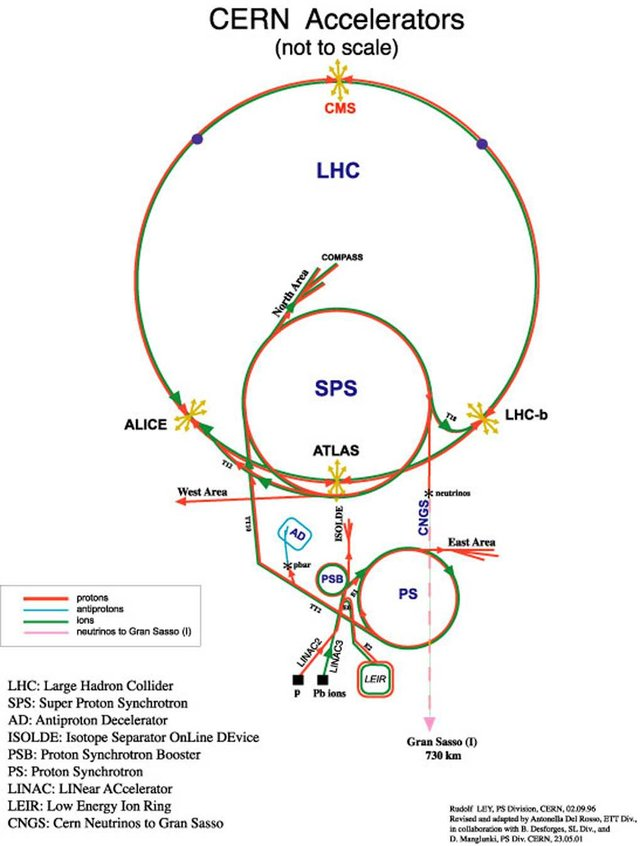
\includegraphics[width=0.9\linewidth]{figures/lhc/injection.jpg}
    \caption{ CERN accelerator complex} 
    \label{fig:injection_chain} 
  \end{center} 
\end{figure}

We begin with the most common element in the Universe, hydrogen, as our source
of protons.  A bottle of hydrogen gas provides 100 microsecond pulses of raw
$H_{2}$ which is then injected into a Duoplasmatron. There,  a strong electric
field and free elctrons from a cathode ionize the molecule into bare $H^{+}$ aka
a proton!  These protons are then accelerated by a 90kV field, leaving the
Duoplasmatron with 1.4\% speed of light ($\sim$4000km/s) or, in relativistic
units, about 83KeV. The bare protons are then fed into the accelerating
RadioFrequency (RF) cavities of Linear Accelerator 2 (LINAC2). Inside,
conductors charged by a powerful oscillating electromagnetic field accelerate
the protons resulting in a 50MeV energy. Along the way, small quadrupole magnets
shape the proton packet insuring they remain in a tight beam.  This pattern of
accleration with RF cavities and shaping/turnig with magnets is then repeated
with CERN's first synchrotron, the Proton Synchrotron (PS) rendering a 1.4 GeV
beam.  The final step before the LHC comes with the Super Proton Synchrotron
where the same technologies are implemented to produce 450 GeV protons, ready
for injection into the LHC. A diagramatic representation of this chain can be
seen in \cref{fig:injection_chain} 

In order to produce proton-proton collisions the LHC uses two beams circulating
in opposite directions.  The beams are not continuous, but instead consist of
bunches, or buckets, of $\mathcal{O}(10^{11})$ protons with a spacing of 25ns.
Given the LHC circumference this allows for 3564 buckets, however only 2808 are
filled per beam due to safety requirements and injection limitations.  Each beam
takes 4 minutes and 20 seconds to fill and then an additional 20 minutes to for
the protons to reach their maximum energy of 7 TeV TeV, or 99.99999991\% the
speed of light! Under normal operating conditions these beams can be used for
many hours.
